\emph{Cancer} is an umbrella term to refer to a group of diseases caused by abnormal cell growth in different parts of the body. The accumulation of extra cells usually forms a mass of tissue called a \emph{tumor}. Tumors can be benign or malignant: \emph{benign tumors} are noncancerous, lack the ability to invade surrounding tissue and will not regrow if removed from the body;  malignant or \emph{cancerous tumors} are harmful, can invade nearby organs and tissues (\emph{invasive cancer}), can spread to other parts of the body (\emph{metastasis}) and will sometimes regrow when removed~\cite{WYNTKABreastCancer2012}.

\emph{Breast cancer} is the cancer that forms in tissues of the breast. The two most common types of breast cancer are \emph{ductal carcinoma} and \emph{lobular carcinoma}; these cancers begin in the breast ducts and lobules, respectively (see Fig.~\ref{fig:BreastAnatomy}). Breast cancer \emph{incidence rate}, the number of new cases in a specified population during a year, is the highest of any cancer among American women. Its \emph{mortality rate}, the number of deaths during a year, is also one of the highest of any cancer~\cite{Howlader2014}.

\begin{figure}[h]
	\centering
	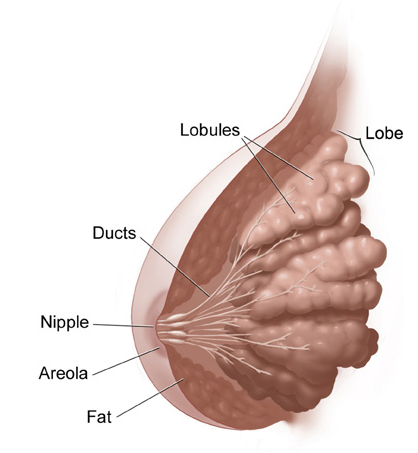
\includegraphics[width = 0.35\textwidth]{plots/breastAnatomy.png}
	\caption[Female Breast Anatomy]{Anatomy of the female breast. Image courtesy of NCI.}
	\label{fig:BreastAnatomy}
\end{figure}

The \emph{cancer stage} depends on the size of the tumor and whether the cancer cells have spread to neighboring tissue or other parts of the body. It is expressed as a Roman numeral ranging from 0 through IV; stage I cancer is considered \emph{early-stage breast cancer} and breast cancer at stage IV is considered \emph{advanced}. Stage 0 describes non-invasive breast cancers, also known as \emph{carcinoma in situ}. Stage I, II and III describe invasive breast cancer, i.e., cancer that has invaded normal surrounding breast tissue. Stage IV is used to describe metastatic cancer, i.e., breast cancer has spread beyond nearby tissue to other organs of the body.
\subsubsection{Mammograms}
A \emph{mammogram} is an x-ray image of the breast. \emph{Screening mammograms} (normally composed of two mammograms of each breast) are used to check for breast cancer signs on women who have not shown symptoms of the disease. If an abnormality is found, a \emph{diagnostic mammogram} is ordered, these are detailed x-ray pictures of the suspicious region~\cite{Mammograms2014}. A standard mammogram is shown in Fig.~\ref{fig:normalMammogram}.

\begin{figure}[h]
	\centering
	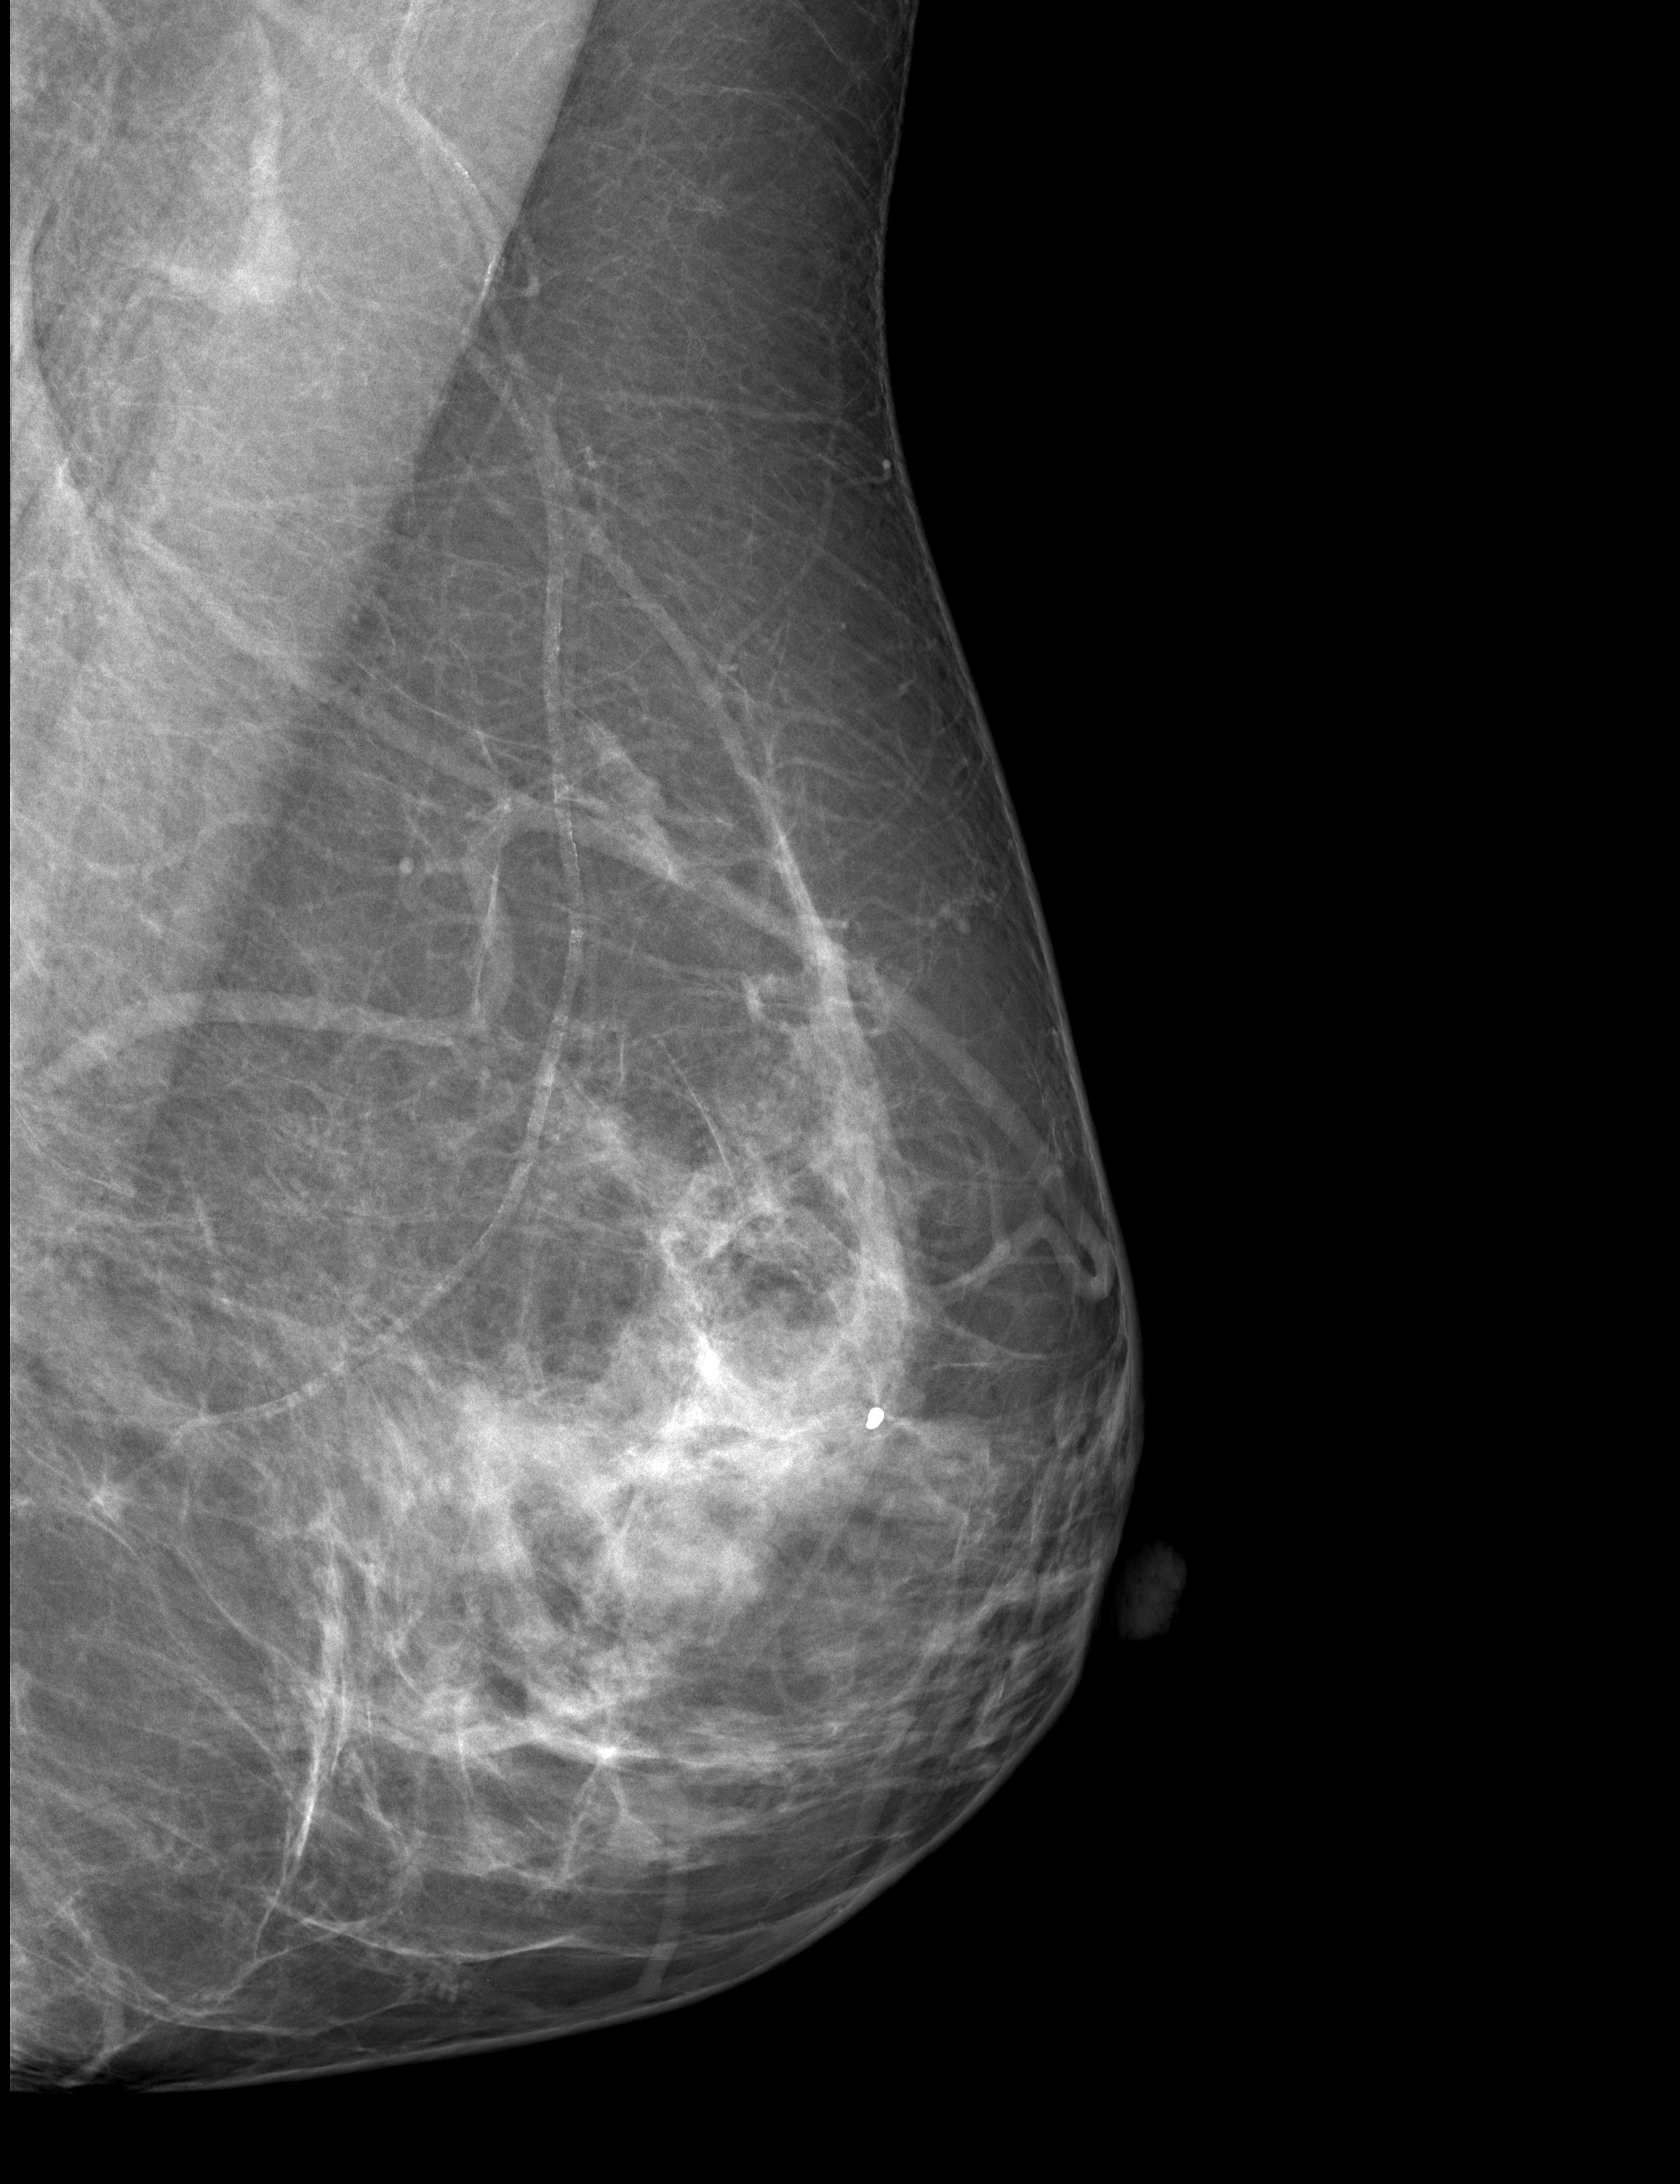
\includegraphics[width = 0.25\textwidth]{plots/normalMammogram.jpg}
	\caption[Digital Mammogram]{A standard mammogram.}
	\label{fig:normalMammogram}
\end{figure}

Having a screening mammogram in a regular basis is the most effective method for detecting early breast cancer; around 85\% of breast cancers can be detected in a screening mammogram~\cite{PerformanceMammography2013}. Nevertheless, screening mammograms have many limitations: a high false positive rate, overtreatment in Stage 0 cancer, false negative results for women with high breast density, radiation exposure and physical and psychological discomfort~\cite{Mammograms2014}.

Mammograms are read by expert radiologists. The radiologist looks primarily for microcalcifications and breast masses. \emph{Microcalcifications} are tiny deposits of calcium in the breast tissue which can be a sign of early breast cancer if found in clusters with irregular layout and shapes. \emph{Breast masses} or breast lumps are possibly a variety of things: fluid-filled cysts, fatty tissues, fibric tissues, noncancerous or cancerous tumors, among others. A mass can be a sign of breast cancer if it has an irregular shape and poorly defined margins. See Fig.~\ref{fig:breastCancerSigns} for an example of possible signs of breast cancer. Radiologists will also consider the breast density of the patient when reading a mammogram given that high breast density is linked to a higher risk of breast cancer and it also difficults the interpretation of the mammogram~\cite{MammogramsACS2014}.

\begin{figure}[h]
	\centering
	\begin{subfigure}{0.25\textwidth}
                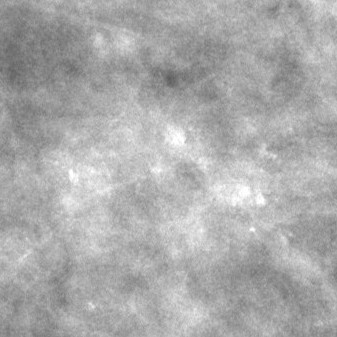
\includegraphics[width=\textwidth]{plots/breastMicrocalcification.jpg}
        \end{subfigure}
	~
	\begin{subfigure}{0.25\textwidth}
                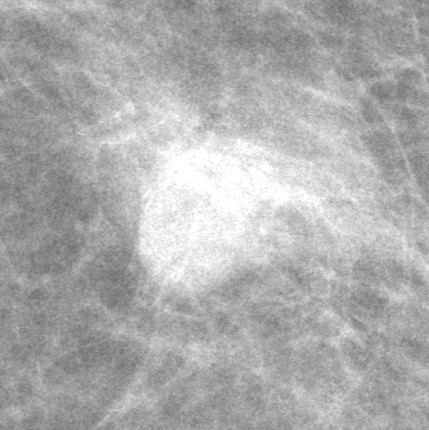
\includegraphics[width=\textwidth]{plots/breastMass.jpg}
        \end{subfigure}
	\caption[Breast Cancer Signs]{Signs of possible breast cancer in a mammogram. Left: A cluster of microcalcifications in an irregular layout. Right: A poorly defined breast mass.}
	\label{fig:breastCancerSigns}
\end{figure}

Conventional mammography uses film to record x-ray images of the breast. \emph{Digital mammography}, on the other hand, uses digital receptors to convert the x-rays into electric signals and stores the image electronically. Digital mammograms offer a clearer picture of the breast and can be digitally manipulated and shared between health care providers. Its effectiveness to identify breast cancer over film mammograms, however, is still debated~\cite{Kerlikowske2011, Pisano2008, Skaane2007}. Digital mammography is steadily becoming the standard for breast cancer screening, Fig.~\ref{fig:normalMammogram} is, in fact, a digital mammogram.

\emph{Digital tomosynthesis}, also called three-dimensional mammography, is a new technology that essentially produces 3-dimensional x-ray images of the breast and is expected to improve the efficacy of regular 2-d mammograms. Studies comparing the two techniques have not yet been published, though~\cite{Mammograms2014}.

In this thesis we will center on using mammograms, either digital or manually digitized from film, to detect microcalcifications and masses and predict the likelihood of breast cancer on the patient.

Much of this section was written using information from the National Cancer Institute. We recommend to visit its website (\url{www.cancer.gov}) for more information.
